\documentclass[a4paper,norsk,12pt]{article}
\usepackage{amsmath,amssymb,amsthm}
\usepackage{graphicx}
\usepackage[norsk]{babel}
\usepackage[utf8]{inputenc}
\usepackage{float}
\usepackage{bm}
\usepackage{titling}
\usepackage{color}
\usepackage{verbatim}
\usepackage{listings}

\lstset{language=c++}
\lstset{alsolanguage=[90]Fortran}
\lstset{basicstyle=\small}
\lstset{backgroundcolor=\color{white}}
\lstset{frame=single}
\lstset{stringstyle=\ttfamily}
\lstset{keywordstyle=\color{red}\bfseries}
\lstset{commentstyle=\itshape\color{blue}}
\lstset{showspaces=false}
\lstset{showstringspaces=false}
\lstset{showtabs=false}
\lstset{breaklines}

\title{\vspace{-4.0cm} \textbf{Obligatorisk innlevering 2, FYS1120-Elektromagnetisme}}
\author{Av: Laila Andersland}

\begin{document}
\maketitle

\textbf{Oppgave 2a}

Elektronet påvirkes av en magneisk kraft 

$$ \textbf{F}_{B} = q ( \textbf{v} \times \textbf{B} ) $$

Vi skal bruke Euler Cromer's metode til å finne bevegelsen til 

elektronet [1].

$$ v(t_i + \Delta t)\simeq v(t_i) + a(t_i , x(t_i) , v(t_i)) \Delta t $$
$$ x(t_i + \Delta t) \simeq x(t_i) + v(t_i + \Delta t) \Delta t $$

\vspace{5mm}

For å finne akselerasjonen må vi bruke sammenhengen: 
$$ \textbf{F}_{B} = q ( \textbf{v} \times \textbf{B} ) $$

hvor vi har alle verdier og kan finne akselesjonenen med $ a = \frac{F}{m_e} $. 

Bruker python for å løse oppgaven numerisk. 

\vspace{5mm}

Implementerer den numeriske metoden i python og får følgende plot:

\begin{figure}[H]
\begin{center}
  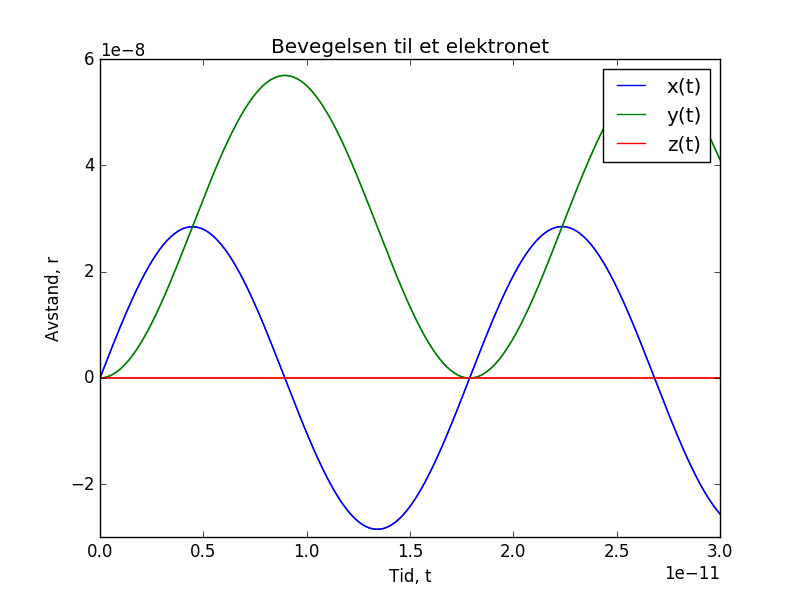
\includegraphics[width=100mm]{oppgave21.png}
  \caption{Plot av bevegelsen til elektronet i x,y,z-retning når plassert i et magnetisk felt.}
  \label{fig:plot1}
  \end{center}
\end{figure}

Figur \ref{fig:plot1} viser at elekronet beveger seg i sirkler i x og y retning for økende tid, t, mens den ikke beveger seg i z-retning. Dette er fordi det magnetiske feltet, som oppgitt i oppgaven kun virket i z-retning, og startsfarten var kun i x retning. Kryssproduktet av disse to gir en akselerasjon i y retning. Elektronet har allerede en fart i x-retning som gir bevegelsen i den retningen, mens z hadde verken en startsfart, eller akselerasjon blir påvirket av det magnetiske feltet. 


\begin{figure}[H]
  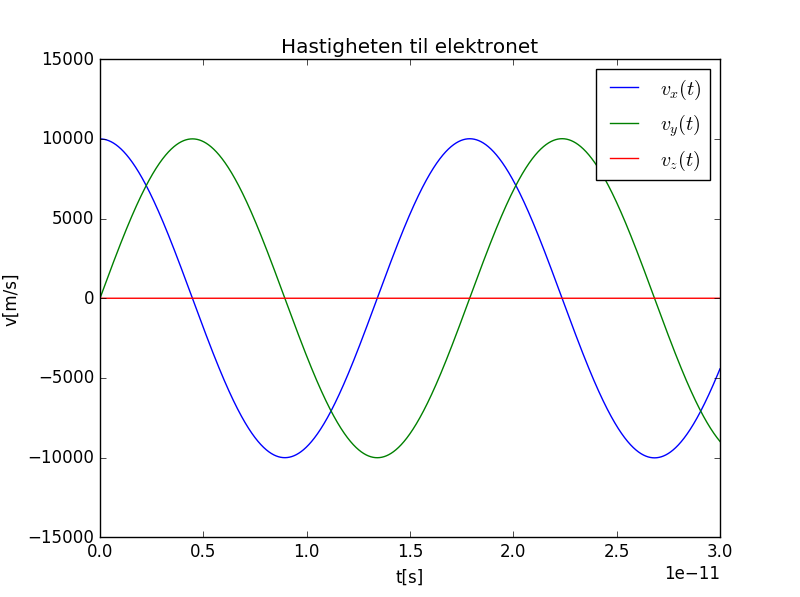
\includegraphics[width=\linewidth]{oppgave22.png}
  \caption{Plot av hastigheten til elektronet i x,y,z-retning når plassert i et magnetisk felt, .}
  \label{fig:plot2}
\end{figure}

I Figur \ref{fig:plot2} ser vi som forventet, ingen hastighet i z-retning, mens hastigheten til partikelen varierer mellom $ \pm 10km/s$. 


\begin{figure}[H]
  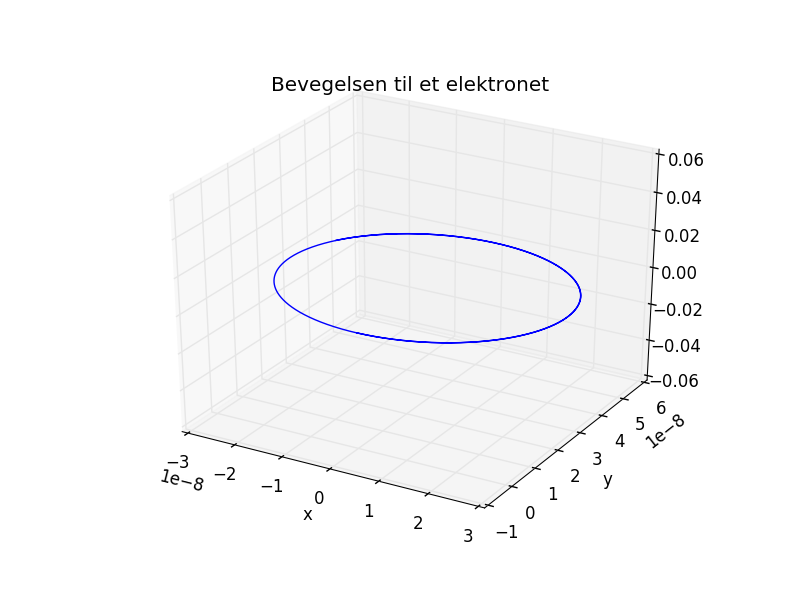
\includegraphics[width=\linewidth]{oppgave23.png}
  \caption{Plot av beveglesen til elektronet i 3D.}
  \label{fig:plot3}
\end{figure}

\textbf{Oppgave 2b}

For å finne omløpstiden kan man vurdere plottet i x-,y-retning:

\begin{figure}[H]
  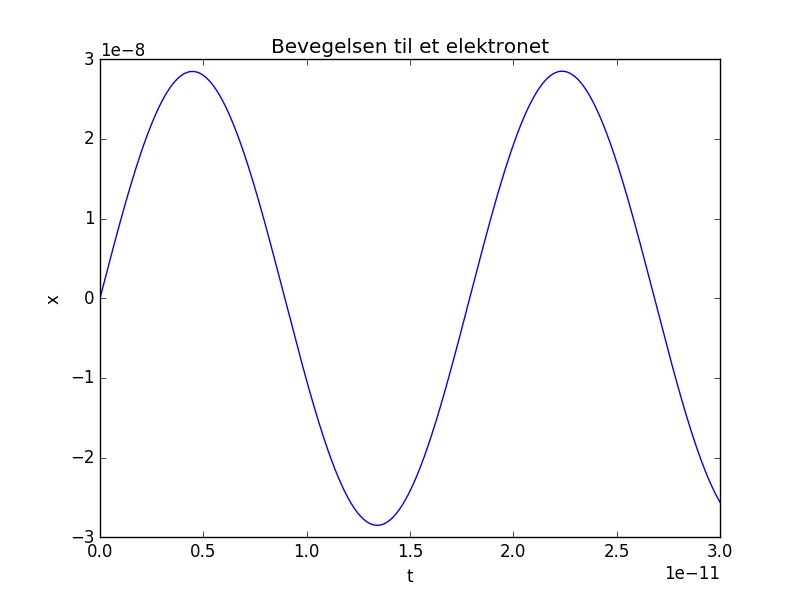
\includegraphics[width=\linewidth]{oppgave24.png}
  \caption{Plot av beveglesen til elektronet i x-retning.}
  \label{fig:plot4}
\end{figure}

I Figur \ref{fig:plot2} kan man se at elektronet bruker omtrent $ 1.75 \times 10^{-11}$ på en 

bølgelengde. 

\hspace{1cm}

\textbf{Oppgave 2c}:

Kraften fra magnetfeltet, $F_M = q v B$, er det samme som 

sentripeltalkraften, $F_S = m \dfrac{v^2}{R}$, hvor $\dfrac{v^2}{R}$ er sentripetalakselrasjonen, slik 

at:

$$ q v B = m \dfrac{v^2}{R} $$ 

Stokker om og får et uttrykk for $R$ som er radiusen til den sirkulære 

banen i magnetfeltet:

$$ R = \dfrac{m v}{q B} $$ 

Bruker $ v = R \omega $ for å finne vinkelfarten:

$$ \omega =  \dfrac{v}{R} =  \dfrac{v}{{m v}/{q B}} =\dfrac{q B}{m} $$

Vinkelfrekvens: $\omega = \dfrac{2 \pi}{T}$

Løser for perioden, T, og setter inn for vinkelfrekvensen, $\omega$:

$$ T = \dfrac{2 \pi}{\omega} = \dfrac{2 \pi}{{q B}/{m}} = \dfrac{2 \pi m}{{q B}}$$

Hvis vi setter inn for T får vi:

$$ T = \dfrac{2 \pi m}{{q B}} =  \dfrac{2 \pi \cdot 9.11 \cdot 10^{-31}}{{{1.6 \cdot 10^{-19}} \cdot 2}} = 1.7887 \cdot 10^{-11}$$

Som er ganske likt den avleste verdien jeg fikk fra plottet i oppgave b.

\hspace{1cm}

\textbf{Oppgave 2d}

Endrer initalhastigheten til $ \textbf{v}(t=0) = (5 000 m/s,0,200 m/s) $ :

\begin{figure}[H]
  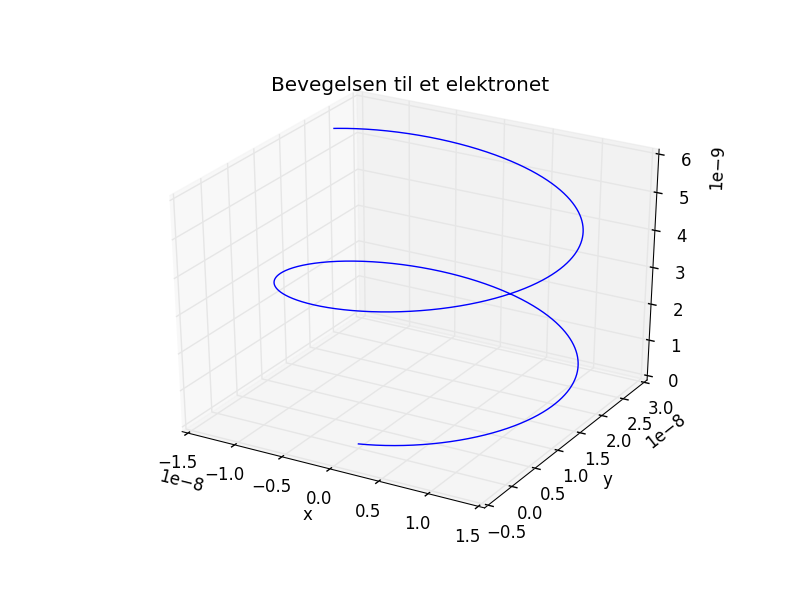
\includegraphics[width=\linewidth]{oppgave25.png}
  \caption{Plot av beveglesen til elektronet med endret initialbetingelser.}
  \label{fig:plot5}
\end{figure}

\textbf{Oppgave 3a}

\begin{figure}[H]
  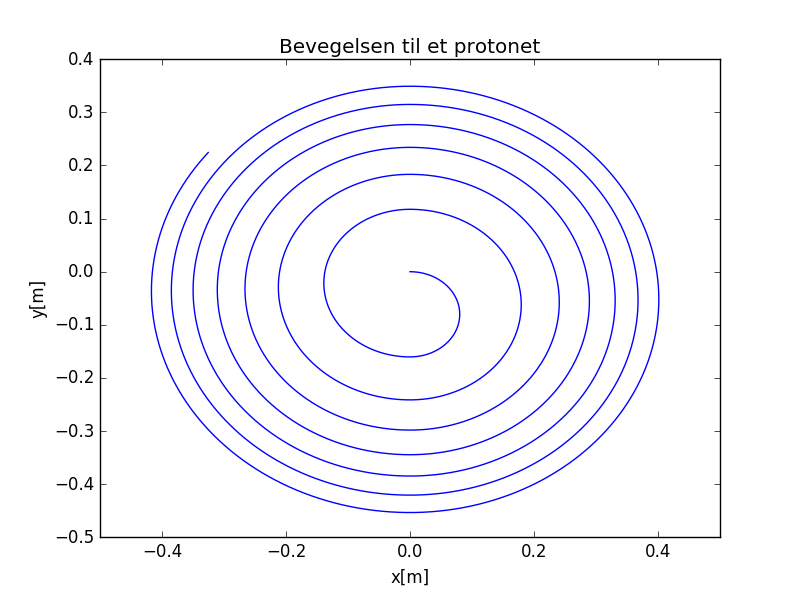
\includegraphics[width=\linewidth]{oppgave31.png}
  \caption{Plot av bevegelsen til protonet i en syklotron.}
  \label{fig:plot6}
\end{figure}

\textbf{Oppgave 3b}

\begin{figure}[H]
  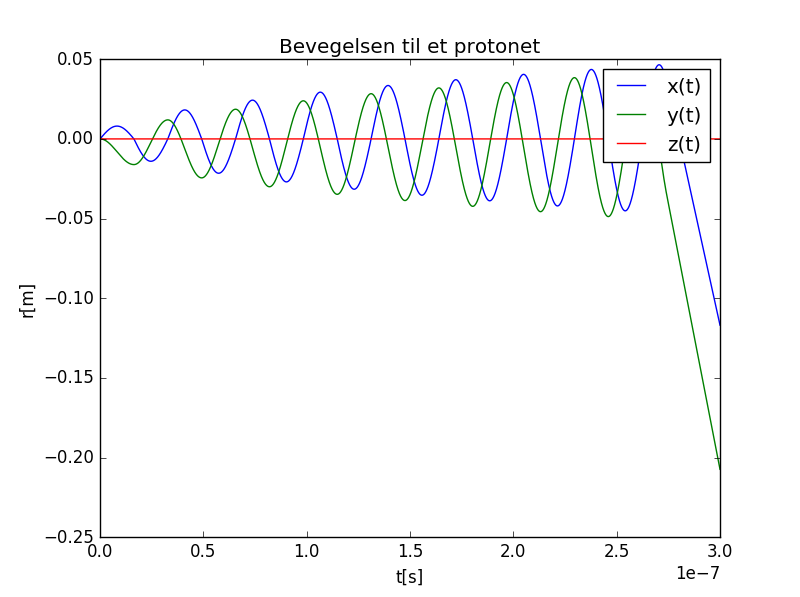
\includegraphics[width=\linewidth]{oppgave32.png}
  \caption{Plot av bevegelsen til protonet i en syklotron.}
  \label{fig:plot7}
\end{figure}


\begin{figure}[H]
  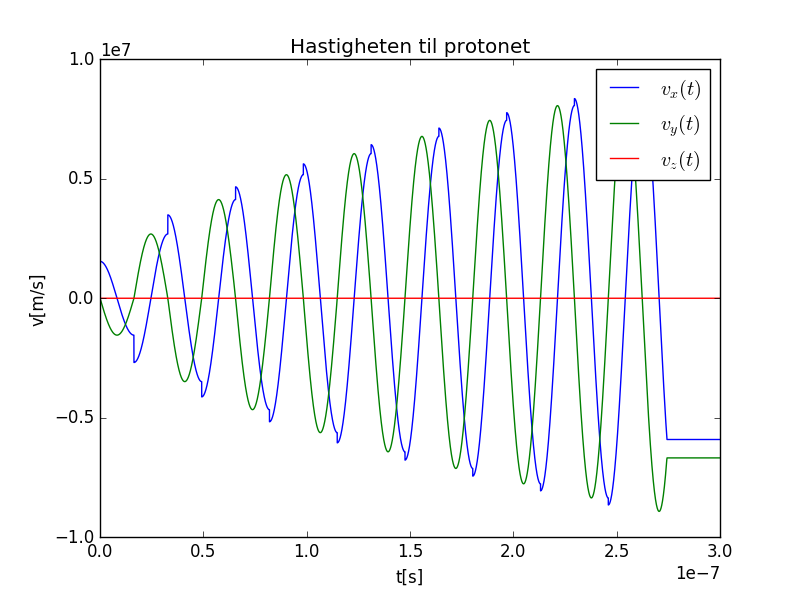
\includegraphics[width=\linewidth]{oppgave33.png}
  \caption{Plot av hastigheten til protonet i en syklotron.}
  \label{fig:plot8}
\end{figure}

\hspace{1cm}

\textbf{Oppgave 3c}

Protonet har tilslutt en fart:  0.00297299911267

\hspace{1cm}

\textbf{Oppgave 3d}

For å finne den kinetiske energien bruker jeg:


\begin{equation}
\label{eq:kinetic}
{ E_k = \dfrac{1}{2} m v^2 }
\end{equation}

Bruker så uttrykket jeg fant for radiusen banen i et sirkulært 

magnetfelt:

$$ R = \dfrac{m v}{q B} $$ 

Løser for farten:

\begin{equation}
\label{eq:speed}
{v = \dfrac{R q B}{m}} 
\end{equation}


Setter så (\ref{eq:speed}) inn i (\ref{eq:kinetic}):

\begin{equation}
\label{eq:Ek}
{ E_k = \dfrac{1}{2} m v^2 } =  \dfrac{1}{2} m (\dfrac{q r B}{m})^2  =  \dfrac{1}{2} \dfrac{q^2 r^2 B^2}{m} 
\end{equation}

\hspace{1cm}

\textbf{Oppgave 3e}

Siden vi vet godt hva vi er ute etter her velger jeg å bruke søkemotoren Scopus for å finne $r_D$ og B. I søkefeltet: , krysser av for vitenskapelige artikler og får:


Her brukes en calley gap, $r_D = 1.47 m$  og Magnetic field range $2.0–4.5 T$ med en Avg. magnetic field range $2.303–3.36 T$

Stokker om på (\ref{eq:Ek}) slik at vi får et uttrykk for massen:


Setter inn for parametrene funnet i artikkelen [].



\hspace{1cm}

\lstinputlisting{Oblig22.py}

\hspace{1cm}

\textbf{Oppgave 4}

Gauss lov:

$$ \Phi_E = \oint \textbf{E} \times d \textbf{A} = \dfrac{Q}{\epsilon_0}$$

\textbf{Oppgave 4a}

\begin{figure}[H]
\centering
  \includegraphics[width=\linewidth, trim={5cm 17cm 5cm 5cm},clip, width=0.5\textwidth,]{illustra4.pdf}
  \caption{Illustrasjon av et gauss-felt lagt koentrisk på innsiden av en kule.}
  \label{fig:plot10}
\end{figure}

Siden kulen er uniformt ladet kan vi formulere en ladningstetthet $\rho$ inne i gaussflaten slik at: 

$$ q = \rho \cdot \dfrac{4}{3} \pi r^{3} $$

Fra Gauss lov får vi da:

$$ \Phi = E(r) \cdot 4 \pi r^2 = \dfrac{q(r)}{\epsilon_0} $$

$$ = E(r) \cdot 4 \pi r^2 = \rho \dfrac{4}{3} \pi r^3 \cdot \dfrac{1}{\epsilon_0} $$

$$ E(r) = \dfrac{1}{4 \pi \epsilon_0 \cdot \dfrac{Q_r}{R^43}} $$

$$ E(r) = \dfrac{1}{4 \pi \epsilon_0} \cdot \dfrac{Q_r}{R^3} $$

\textbf{Oppgave 4b}

\begin{figure}[H]
\centering
  \includegraphics[width=\linewidth, trim={1cm 15cm 1cm 5cm},clip, width=0.5\textwidth,]{illustra6.pdf}
  \caption{Illustrasjon av et $\infty$-liggende ark med et gauss-felt i form av en eske over.}
  \label{fig:plot11}
\end{figure}

$$ \Phi = E s^2 \cdot 2 = \dfrac{q}{\epsilon_0} = \dfrac{\sigma a^2}{\epsilon_0} $$

\textbf{Oppgave 4c}

\begin{figure}[H]
\centering
  \includegraphics[width=\linewidth, trim={1.5cm 13cm 5cm 2cm},clip, width=0.5\textwidth,]{illustra5.pdf}
  \caption{Illustrasjon av et gauss-felt lagt rundt en uniformt ladet stav.}
  \label{fig:plot12}
\end{figure}

$$ \Phi = \oint \textbf{E} \cdot d \textbf{A} = \dfrac{Q}{\epsilon_0} $$

Hvor: $ \lambda = \dfrac{Q}{L}$ og  $ \lambda \cdot H = q_{inni} $

$$ \textbf{E} (r) \cdot 2 \pi r \cdot H = \dfrac{\lambda H}{\epsilon_0} $$

Og får:

$$ E(r) = \dfrac{\lambda}{2 \pi r \epsilon_0} $$

\medskip
 
\begin{thebibliography}{9}
 
\bibitem{einstein} 
Anders Malthe-Sørensen. 
\textit{Elementary Mechanics Using python}. 
Springer, ISBN 978-3-319-19595-7, 2015.
 
\bibitem{knuthwebsite} 
Knuth: Computers and Typesetting,
\\\texttt{http://www-cs-faculty.stanford.edu/\~{}uno/abcde.html}
\end{thebibliography}


\end{document}